\hypertarget{ProbabilisticClustering_8c_09_09}{
\section{src/expmax/ProbabilisticClustering.c++-\/Dateireferenz}
\label{ProbabilisticClustering_8c_09_09}\index{src/expmax/ProbabilisticClustering.c++@{src/expmax/ProbabilisticClustering.c++}}
}
{\ttfamily \#include \char`\"{}ProbabilisticClustering.h++\char`\"{}}\par
{\ttfamily \#include $<$typeinfo$>$}\par
{\ttfamily \#include $<$boost/foreach.hpp$>$}\par
{\ttfamily \#include $<$boost/optional.hpp$>$}\par
{\ttfamily \#include $<$boost/mpl/equal.hpp$>$}\par
{\ttfamily \#include $<$boost/function.hpp$>$}\par
{\ttfamily \#include $<$boost/lambda/bind.hpp$>$}\par
{\ttfamily \#include $<$boost/lambda/lambda.hpp$>$}\par
{\ttfamily \#include $<$algorithm$>$}\par
{\ttfamily \#include $<$boost/iterator/counting\_\-iterator.hpp$>$}\par
{\ttfamily \#include $<$boost/algorithm/minmax\_\-element.hpp$>$}\par
{\ttfamily \#include $<$boost/shared\_\-ptr.hpp$>$}\par
{\ttfamily \#include $<$boost/numeric/ublas/matrix.hpp$>$}\par
{\ttfamily \#include $<$boost/numeric/ublas/symmetric.hpp$>$}\par
{\ttfamily \#include $<$boost/numeric/ublas/vector.hpp$>$}\par
{\ttfamily \#include $<$boost/numeric/ublas/vector\_\-proxy.hpp$>$}\par
{\ttfamily \#include $<$boost/numeric/ublas/io.hpp$>$}\par
{\ttfamily \#include $<$boost/numeric/ublas/lu.hpp$>$}\par
{\ttfamily \#include $<$limits$>$}\par
{\ttfamily \#include $<$iostream$>$}\par
{\ttfamily \#include \char`\"{}math/CircularStatistics.h++\char`\"{}}\par
{\ttfamily \#include \char`\"{}math/numeric\_\-optimization.h++\char`\"{}}\par
{\ttfamily \#include \char`\"{}utils/comparisons.h++\char`\"{}}\par
{\ttfamily \#include \char`\"{}common\_\-definitions.h++\char`\"{}}\par
{\ttfamily \#include \char`\"{}FitMultivariateMulticlassByEM.h++\char`\"{}}\par
{\ttfamily \#include \char`\"{}EMGenericMixtureModelCore.h++\char`\"{}}\par
{\ttfamily \#include \char`\"{}EMCustomOptimization.h++\char`\"{}}\par
{\ttfamily \#include $<$sstream$>$}\par
{\ttfamily \#include $<$boost/numeric/ublas/triangular.hpp$>$}\par
Include-\/Abhängigkeitsdiagramm für ProbabilisticClustering.c++:\nopagebreak
\begin{figure}[H]
\begin{center}
\leavevmode
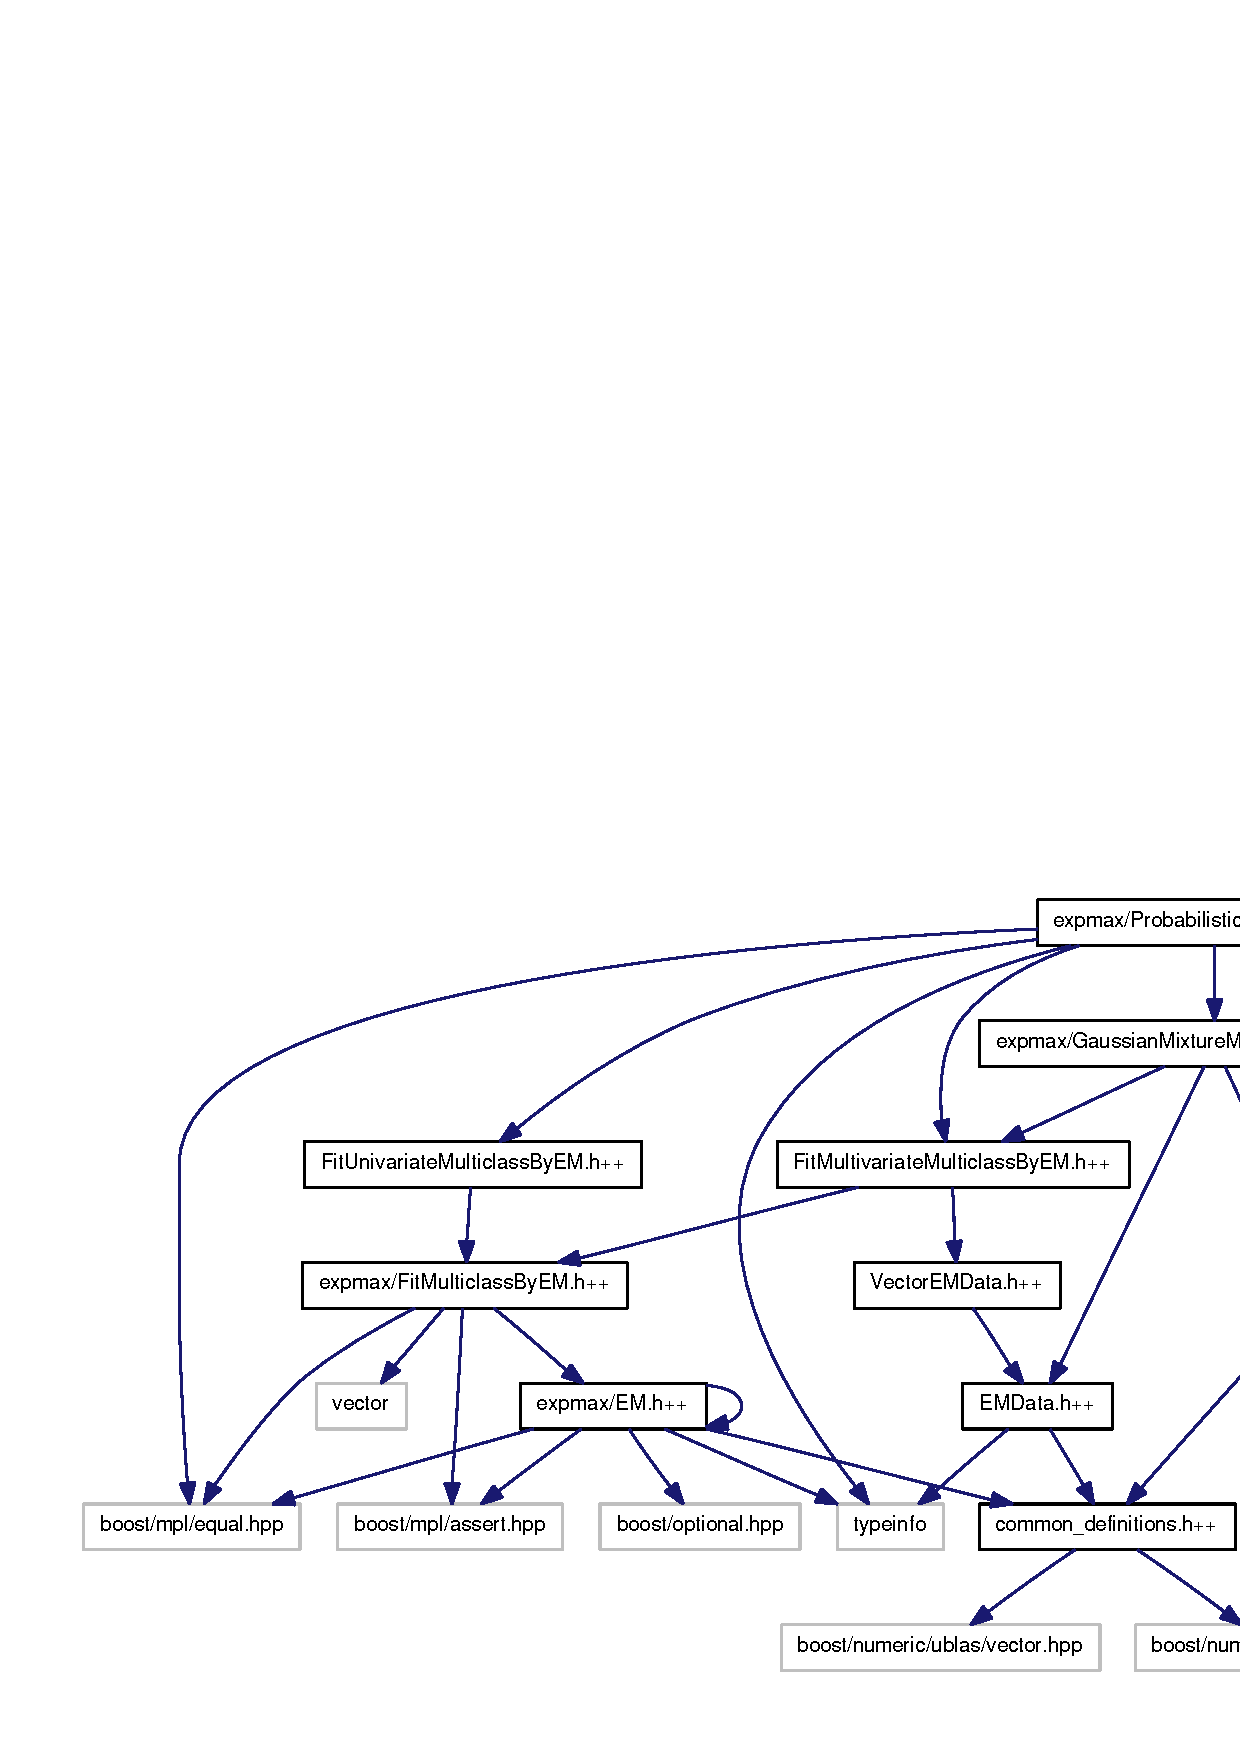
\includegraphics[width=420pt]{ProbabilisticClustering_8c_09_09__incl}
\end{center}
\end{figure}
Dieser Graph zeigt, welche Datei direkt oder indirekt diese Datei enthält:\nopagebreak
\begin{figure}[H]
\begin{center}
\leavevmode
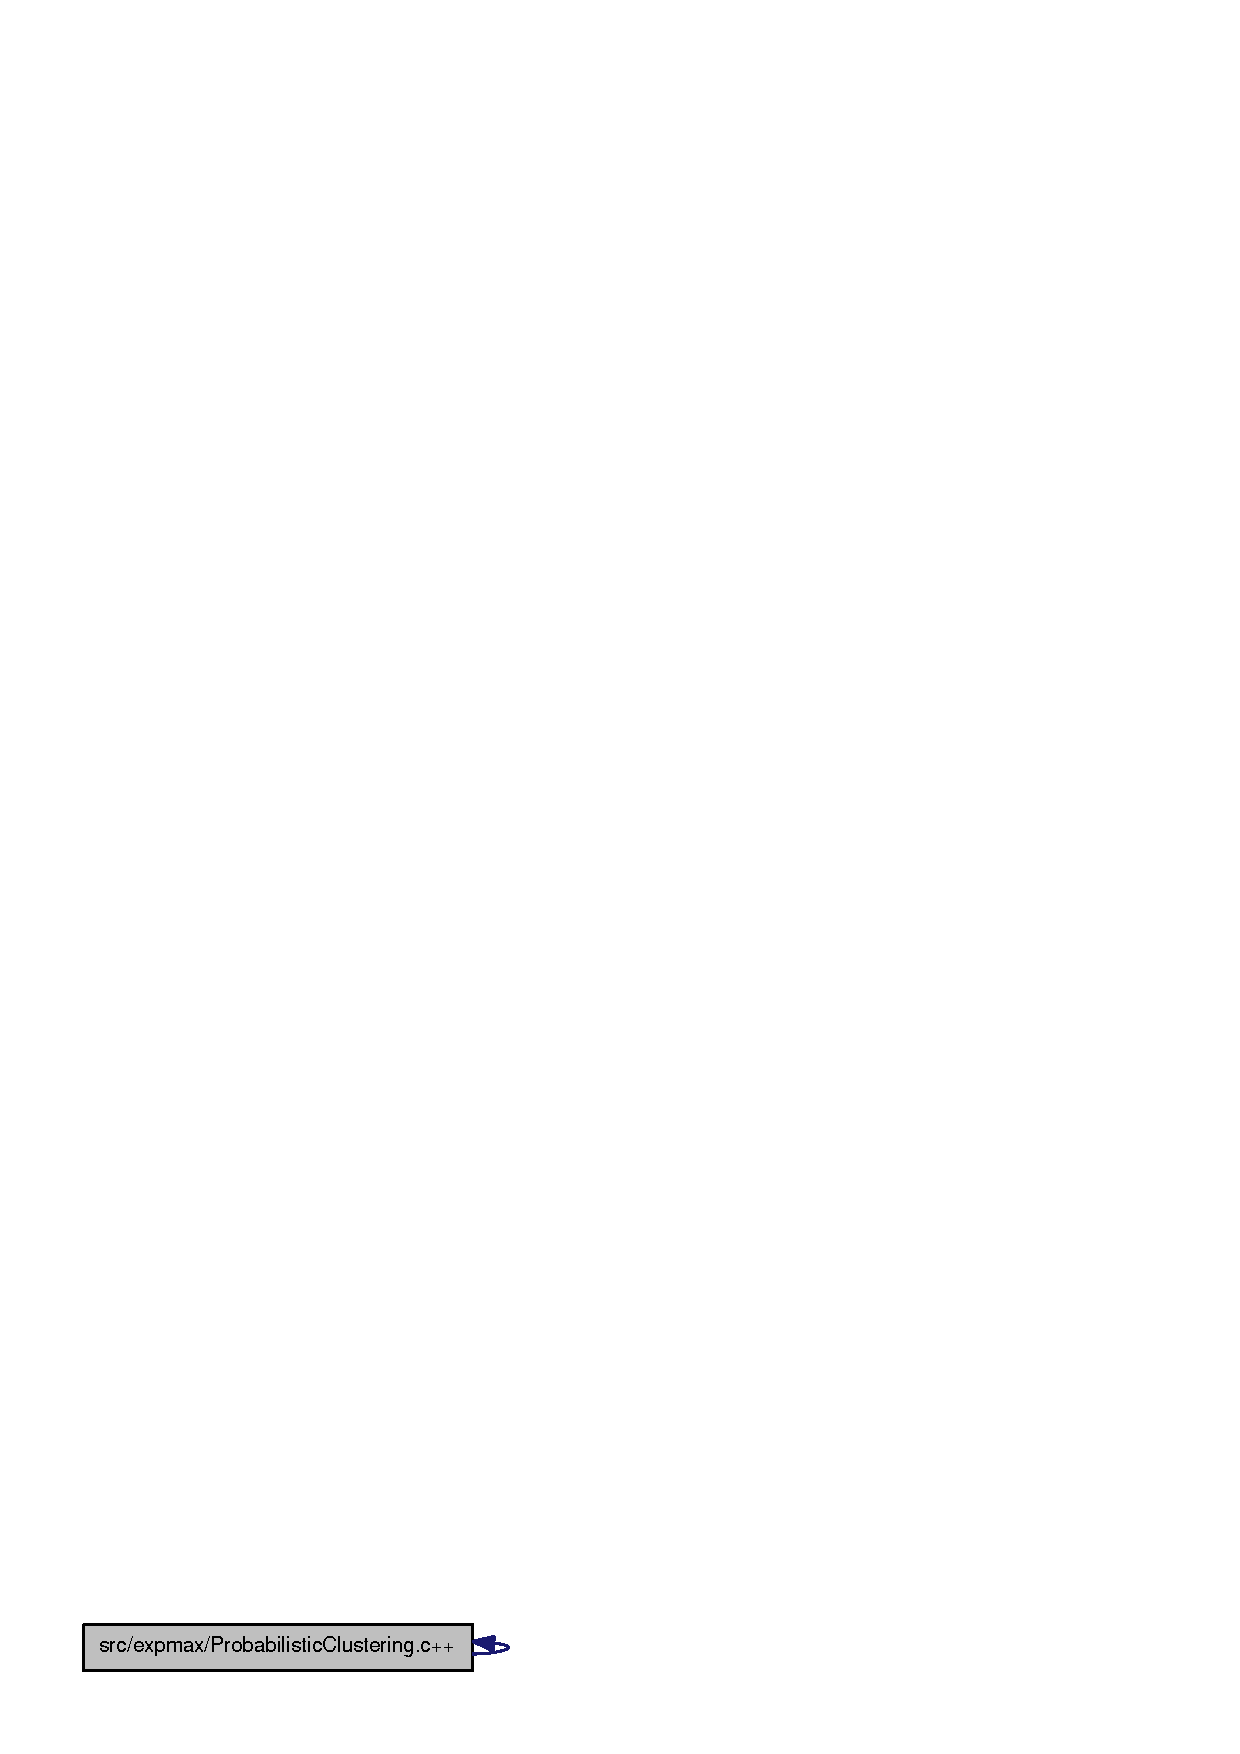
\includegraphics[width=124pt]{ProbabilisticClustering_8c_09_09__dep__incl}
\end{center}
\end{figure}


\subsection{Ausführliche Beschreibung}
\begin{DoxyAuthor}{Autor}
Erik Flick $<$erik.flick \mbox{[}AETT\mbox{]} informatik.uni-\/hamburg.de$>$ 
\end{DoxyAuthor}
\begin{DoxyVersion}{Version}
0.1
\end{DoxyVersion}
\hypertarget{ProbabilisticClustering_8h_09_09_LICENSE}{}\subsection{LICENSE}\label{ProbabilisticClustering_8h_09_09_LICENSE}
This file is released under LGPL v3.0.

Created on: Dec 16, 2010

\begin{Desc}
\item[\hyperlink{todo__todo000007}{Noch zu erledigen}]crippling bugs in multivariate gaussian specialization\end{Desc}
